\section{Sunquakes}
\subsection{Introduction}
%Chronological soft intro; use some of the lit review,
%making sure to emphasize the connection to solar flares;Look at early papers predicting sunquakes(Wolff 70s and Kosovichev and Zharkova);the importance of sunquakes


During this age of space-born solar astronomy, understanding the highly dynamic environment of the Sun's atmosphere is a study enriched by a wealth of high detail observations. With each newly launched space instrument the spatial resolution of collected data increases, which coupled with those spacecraft that are tailored to capture light of previously unobserved wavelengths, often leads to new phenomena being observed. Eruptive solar flares fall into this category, in that spacecraft have provided observations that challenge the current theoretical view that the standard eruptive flare model (CSHK model: \citep{1964NASSP..50..451C, 1966Natur.211..695S, 1974SoPh...34..323H, 1976SoPh...50..} puts forward. 

Solar flares are one of the most energetic events to occur in the Sun's atmosphere, where by stored magnetic energy is released in the form of heat, mass motions, and accelerated particles. This highly dynamic process produces many measurable signatures, such as emission from $\gamma$-ray to optical wavelengths, a high percentage of which agree with the CSHK model, however, this is not the full picture. The standard flare model has been modified to include new observations many times over the years \citep{2011LRSP....8....6S} and is still unable to describe some observed phenomena. Therefore there is still work to be done before a true account of the complex nature of solar flares are to be realised.    

Sunquakes are an observable feature during some solar flares that the standard model is unable to explain. It is believed that they are the result of energy and momentum released during the flare impacting the lower solar atmosphere. During a solar flare, energy is released high up in the solar atmosphere and transported down to lower altitudes. If a sufficient amount of energy impacts the lowest atmospheric layer, then acoustic waves are produced which propagate into sub-surface layers of the Sun producing a sunquake (see figure \ref{sunquake-cartoon}a). As acoustic wavefronts travel into the interior they encounter layers of increasing density causing refraction back toward the solar surface (see figure \ref{sunquake-cartoon}b). At which point, waves can be observed as circular formations in the surface plasma , expanding outward from a point of origin (see Figure \ref{mdiquake96}). 


\begin{figure}\label{sunquake-cartoon}
  \begin{center}
  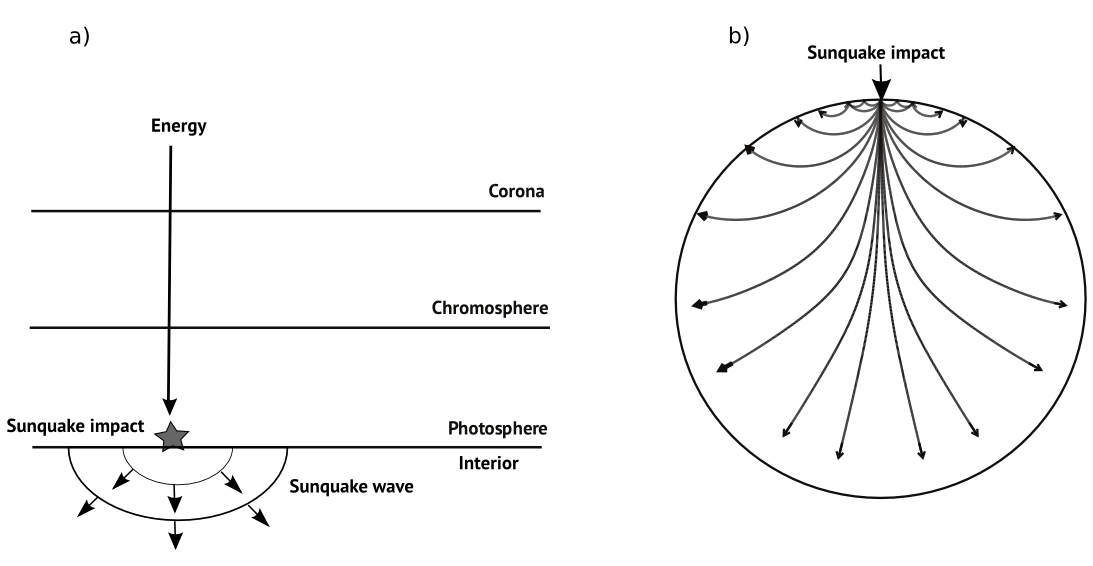
\includegraphics[width=0.40\textwidth]{sunquake-cartoon}
  \end{center}
  \caption{Sunquake cartoon: a) Shows a basic picture of sunquake production. Energy moves down through the solar atmosphere impacting the photosphere and generating a sunquake. b) Shows acoustic wavefronts propagating into the interior of the Sun. Wavefronts refract back toward the surface as they encounter increasingly dense sub-surface layers. Waves reaching the surface disturb material in a pattern resembling ripples in a pond.}
\end{figure}

\subsection{Sunquake Observations}
The possability that solar flares cause acoustic waves inside the Sun was originally put forward by \citep{1972ApJ...176..833W}. Wolff made the connection that a large solar flare releasing enough energy to heat the photosphere, would generate expansion of photospheric material, which could lead to an impulsive stimulation of oscillations in the Sun's interior. Wolff also commented that it would be difficult to observe interior oscillations with current solar velocity measurement techniques.      

A little over twenty years later and Wolff's idea was built upon by \cite{1995ESASP.376b.341K}, who showed theoretically that acoustic waves in the solar interior could be generated by a large solar flare, and that they may be detectable. A year later and the first detection of a sunquake was made by \cite{1998Natur.393..317K} during an X class solar flare on July the 9th 1996. Their observational data came from the Solar and Heliospheric Observatory (SOHO) via the Michelson Doppler Imager (MDI) which images the movement of photospheric material by analysing shifts in wavelength of the emitted light. They observed a prominent impulsive downward signature in the Dopplergrams directly over a compact point source emanating a set of concentric acoustic waves (see Figure \ref{mdiquake96}. The timing of maximum downward velocity of material derived from the Dopplergrams was out of sync with peak hard x-ray measurements by around a minute. This time delay, coupled with white-light enhancement in the lower atmosphere led to the conclusion that during the flare, accelerated energetic particles heat the cool dense chromosphere causing a shock front which travels downward, depositing energy in lower atmospheric layers, generating a sunquake. 
 
\begin{figure}\label{mdiquake96}
  \begin{center}
  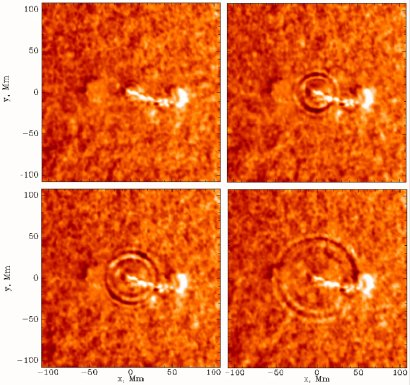
\includegraphics[width=0.40\textwidth]{soho-mdi-quake-96}
  \end{center}
  \caption{\cite{1998Natur.393..317K} produced SOHO MDI Dopplergrams from the 1996 July 9th, X class solar flare showing the sunquake evolving over time. Each frame relates to a $####s$ progression in time. The sunquake expands outward from it's seismic epicenter to a radial distance of $1.2\times10^{8}$ metres with a wave amplitude of $###km$ . Wavefronts accelerate over time, propagating with an average velocity of $###km.s^{-1}$ }
\end{figure}


The first sunquake observation opened up a whole new area of solar physics to science, leading to a multitude of detections associated with many different flares. The majority of observations show that sunquakes are often the product of highly impulsive flares, with the acoustic source aligning spatially with white light enhancement in the lower solar atmosphere and hard x-ray emission from the upper-atmosphere \citep{2005ApJ...630.1168D, 2007ApJ...664..573Z}. \cite{2005ApJ...630.1168D} went on to calculate the energy needed to stimulate the propagation of an acoustic wave in the sub-photosphere. The authors found that only $\sim10^{-3}$ of the energy released by a flare is enough to generate a sunquake. This was an important calculation because it forced the solar community to consider that it might be possible for smaller energy flares to produce sunquakes, leading subsequent work (e.g., \cite{2008SoPh..251..613M}) analysing sunquakes from lower energy flares.

A paper by \cite{2000ApJ...531L..75H} put forward for the first time, that sunquake production may depend on the changing configuration of the magnetic field. This idea was further reinforced by \cite{2001ApJ...550L.105K} reporting observations of impulsive changes in magnetic field strength at the photosphere during a solar flare. These magnetic transients were shown to approximately correlate in time and space with hard x-rays and impulsive increases in plasma velocity and emission intensity. This line of study was continued \citep{2009MNRAS.395L..39M}, investigating the magnetic field variation of the photosphere in many flares. The study found that some flares with seismicity do not have a spatial and temporal correlation between sunquakes and magnetic transients. Some flares have magnetic transients and no seismicity, and some flares have a good co-spatial alignment of acoustic activity and magnetic variability. It was noted that the impulsiveness of the magnetic field variation could be important as to whether a sunquake is generated.

Probably the most intriguing of sunquake observations are those that do not abide by the usual set of observable features, in that they are not necessarily associated with hard x-rays and white-light emission. For example, a statistical survey carried out by \cite{2012SoPh..277..317P}, highlighted a flare containing three footpoints with a seismic source that was co-temporal but not co-spatial with it's closest HXR footpoint; and another source which was co-spatial and co-temporal with it's nearest HXR footpoint.

Another example by \cite{2011ApJ...741L..35Z} reports an observation of two seismic sources associated with a flare that erupts producing a coronal mass ejection (CME). During the eruption, the magnetic field above each seismic source undergoes an abrupt permanent reconfiguration. The authors cite the possibility that there exists particle beams low enough in population that HXR emission is undetectable. Further papers investigating the same event \citep{2013SoPh..284..315Z} showing that there are downward motions of material above the seismic sources and that energy provided by magnetic transients may not be able to account for the acoustic power generated.       


